\documentclass[11pt,aspectratio=1610,xcolor=dvipsnames]{beamer}

\usetheme[
    background=light,
    numbering=fraction,
    block=fill,
    progressbar=frametitle
]{metropolis}

\graphicspath{{img/}}

\usepackage[style=authortitle-ibid,backend=biber]{biblatex}
\addbibresource{refs.bib}
\setbeamerfont{footnote}{size=\scriptsize}
\setbeamercovered{transparent}

\usepackage{physics}
\usepackage{mathtools}
\usepackage{bbm}
\usepackage{booktabs}
\usepackage[most,skins,theorems]{tcolorbox}
\tcbset{variables/.style={colback=yellow!20,colframe=yellow}}
\usepackage{tikz}
\usetikzlibrary{shapes.geometric, arrows, shadows}
\usetikzlibrary{fit, backgrounds}



% \colorlet{LightLavender}{Lavender!40!}
\newtcolorbox{prob}{colback=red!5!white,colframe=red!75!black}
\usefonttheme[onlymath]{serif}
\usepackage{quantikz}
\usepackage{qrcode}
\usepackage{pgfplots}
\usepackage{pythonhighlight}

\newcommand{\R}{\mathbb{R}}
\newcommand{\U}[1]{\mathsf{U}(#1)}
\newcommand{\defeq}{\stackrel{\text{\tiny def}}{=}}

\titlegraphic{
\includegraphics[width=0.3\textwidth]{unitary_fund_logo.png}}

\title{Locality and Error Mitigation of Quantum Circuits}
\subtitle{Quantum Wednesday}
\date{Apr 19, 2023}
\author{Nate Stemen}


\begin{document}

\maketitle

\begin{frame}{Today's Paper}
	\begin{figure}[h]
		\centering
		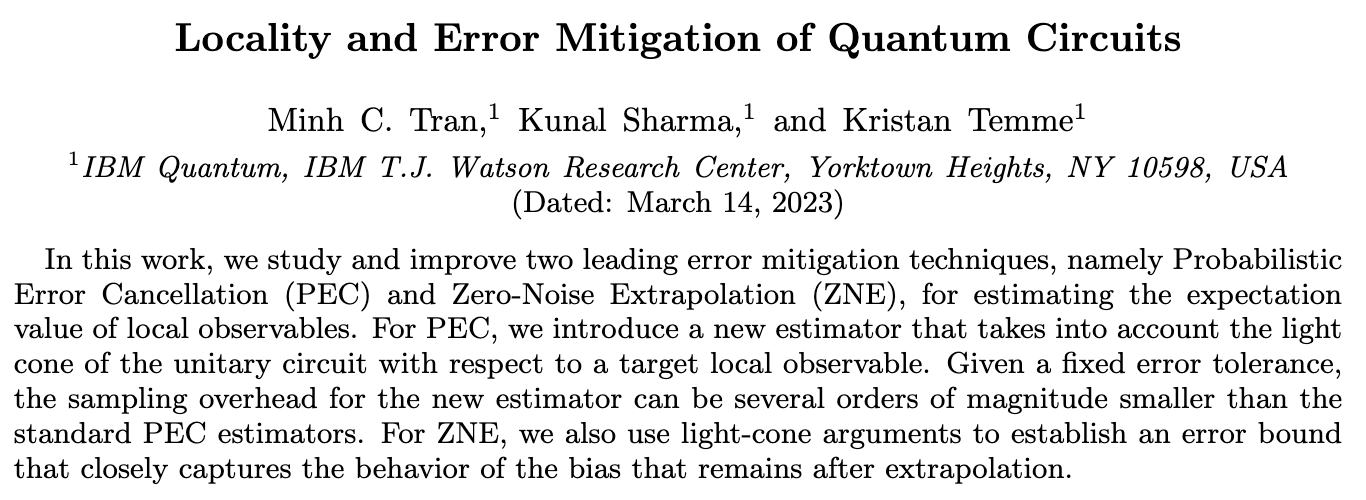
\includegraphics[width=0.8\textwidth]{paper.png}
	\end{figure}
	\begin{center}
		\url{https://arxiv.org/abs/2303.06496}
	\end{center}
\end{frame}

\begin{frame}{Review}
	\begin{columns}
		\begin{column}{0.5\textwidth}
			{\Large Zero-Noise Extrapolation}
			\begin{enumerate}
				\item something
			\end{enumerate}
		\end{column}
		\begin{column}{0.5\textwidth}
			{\Large Probabilistic Error Cancellation}
			\begin{enumerate}
				\item something else
			\end{enumerate}
		\end{column}
	\end{columns}
\end{frame}

\begin{frame}{Key Concepts}
	\begin{columns}
		\begin{column}{0.5\textwidth}
			{\Large Local Observable}
			\begin{enumerate}
				\item something
			\end{enumerate}
		\end{column}
		\begin{column}{0.5\textwidth}
			{\Large Light Cone}
			\begin{enumerate}
				\item something else
			\end{enumerate}
		\end{column}
	\end{columns}
\end{frame}

\begin{frame}{Assumptions}
	\begin{enumerate}
		\item
	\end{enumerate}
\end{frame}

\begin{frame}{What is an observables light cone?}

\end{frame}


\begin{frame}[fragile]{Do we want these techniques in Mitiq?}
	\begin{enumerate}
		\item Does this slot into our existing \verb|execute_with_pec| function?
		\item How does this perform as an observable $O$ go from local to ``unlocal''.
	\end{enumerate}
\end{frame}

\begin{frame}[standout]
	Thank you!
\end{frame}

\end{document}
